\documentclass[paper=a4, fontsize=11pt]{scrartcl}
\usepackage[T1]{fontenc}
\usepackage{fourier}

\usepackage[english]{babel}															% English language/hyphenation
\usepackage[protrusion=true,expansion=true]{microtype}	
\usepackage{amsmath,amsfonts,amsthm} % Math packages

\usepackage{graphicx,subfigure}
%\usepackage[pdftex]{graphicx}	
\usepackage{url}
\usepackage{soul,color}

%%% Custom sectioning
\usepackage{sectsty}
\allsectionsfont{\centering \normalfont\scshape}


%%% Custom headers/footers (fancyhdr package)
\usepackage{fancyhdr}
\pagestyle{fancyplain}
\fancyhead{}											% No page header
\fancyfoot[L]{}											% Empty 
\fancyfoot[C]{}											% Empty
\fancyfoot[R]{\thepage}									% Pagenumbering
\renewcommand{\headrulewidth}{0pt}			% Remove header underlines
\renewcommand{\footrulewidth}{0pt}				% Remove footer underlines
\setlength{\headheight}{13.6pt}


%%% Equation and float numbering
\numberwithin{equation}{section}		% Equationnumbering: section.eq#
\numberwithin{figure}{section}			% Figurenumbering: section.fig#
\numberwithin{table}{section}				% Tablenumbering: section.tab#


%%% Maketitle metadata
\newcommand{\horrule}[1]{\rule{\linewidth}{#1}} 	% Horizontal rule

\title{
		%\vspace{-1in} 	
		\usefont{OT1}{bch}{b}{n}
		\normalfont \normalsize \textsc{Information Retrieval} \\ [25pt]
		\horrule{0.5pt} \\[0.4cm]
		\huge Programming Project - Phase 3 \\
		\horrule{2pt} \\[0.5cm]
}
\author{
		\normalfont 								\normalsize
        Primal Pappachan\\[-3pt]		\normalsize
        primal1@umbc.edu\\[-3pt]		\normalsize
        \today
}
\date{}


%%% Begin document
\begin{document}
\maketitle
\section{Introduction}
In Phase 3 of the project, I have implemented a program which generates the index/inverted file for a given document collection. I have used my code from phase 1 and 2 of the project for tokenizing as well as calculating normalized term weights.  I also evaluated the performance of the code in terms of running time as well as the size of output in comparison to the input. I have used Python to code the entire program. To execute the program from a terminal (after setting right permissions for the file), type 

\begin{verbatim}
$./index input-directory output-directory <n>
\end{verbatim}

The last parameter is optional and specifies the number of files which should be considered from the input directory (default value - 503). You need to install the NLTK to run the program. Please refer to the documentation\footnote{\url{http://www.nltk.org/install.html}} on how to install NLTK.

\paragraph{Output}

The output\_directory contains two output files. Both files are in ASCII. In the first output file named postings file, each line represents a record which denotes the document id and normalized weight of the word in the document for every token that survived preprocessing step. The second output file is a dictionary where records are in alphabetical order. Each record emcompasses three lines and contain the information such as the word, number of documents that contain the word and location of the first record (line number) for that word in the postings file.

\section{Preprocessing and Term weighting}

I used preprocessing code from previous phase albeit with two minor additional constraints on validity of tokens. The size of token should be between 2 and 20 and it should not be a number. For term weighting, instead of writing the results to a file I stored it in a nested hashtable for easier retrieval. The normalized weight of a term could be retrieved using a simple dictionary operation (weights[document][term], where weights is the name of the dictionary).

\section{Building the index}

The index was built by iterating through the nested dictionary. For each term, the id of document which it appears in as well as normalized weight of the term is written to the postings file. A counter variable was used to record the last line number written in file. After going through all documents corresponding to a term, a single entry for that term is stored in a list as tuple (term, document frequency, location of first record in postings file). The document frequency for a term was obtained from the inverse document dictionary (inverse\_doc\_freq[term] returns number of documents that contain that term) built in phase 2. After going through all the tokens, the list of tuples were sorted according in alphabetical order of terms and the result was written to the dictionary file.      

\section{Evaluation}

I ran index on a varying number of documents and plotted a graph of indexing time as a function of the number of documents. The timing was done for the complete process, i.e starting with the raw input files to the generation of two output files. For experiments, I used a macbook air with 8 gb of ram. \\

In the first graph, the real time (elapsed time) taken by the program increases linearly with number of files (except for a slight decrease for 100 files which happened because randomly chosen list of files in that step were smaller in size compared to earlier step as can be seen from size of files graph). With larger number of files (100, 200, 300, 400, 500) the time grows linearly  as well. The system time remains fairly constant throughout the first graph where as it registers a slight increase in the second graph.  \\


\begin{figure}[h]
\centering
\subfigure[10, 20, 40, 80, 100]{ \label{fig:sub1}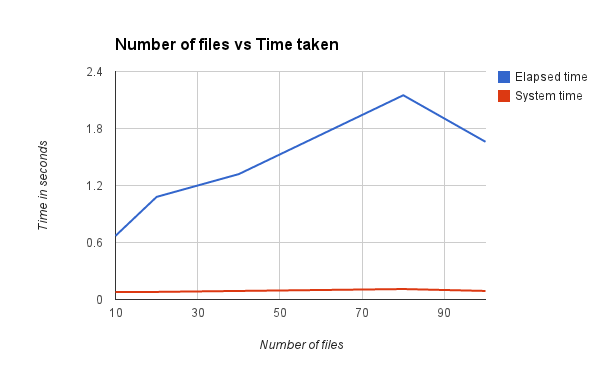
\includegraphics[width=.6\linewidth]{time_1.png}}
\subfigure[100, 200, 300, 400, 500]{ \label{fig:sub2}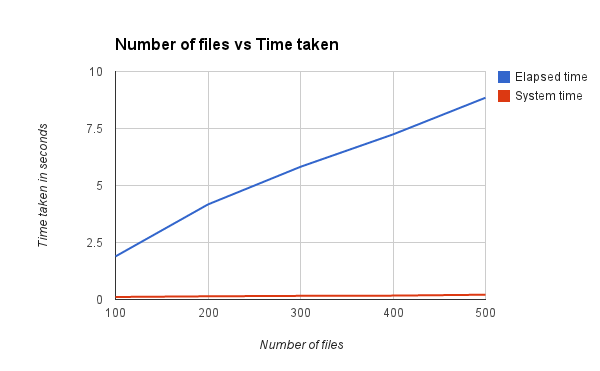
\includegraphics[width=.6\linewidth]{time_2.png}}
\caption{Execution time of index against number of documents}
\end{figure}

Additionally, I also compared the output file sizes against set of input files for different number of files. I used the python function os.path.getsize which returns the file size in bytes which was converted into MB by dividing by 1024*1024. \\

As you can see from the graphs below, the size of the postings file was comparable to that of the input document collection. The size of dictionary was much smaller in comparison. For compressing the postings file, I could use a smaller representation of the document id such as hash value or the just the filename instead of using the entire path for each file which on the flip side makes it easier to retrieve the document. Additionally I could use techniques like variable encoding (variable byte codes, gamma codes)  \cite{comp} for compressing the postings file.   


\begin{figure}[h]
\centering
\subfigure[10, 20, 40, 80, 100]{ \label{fig:sub1}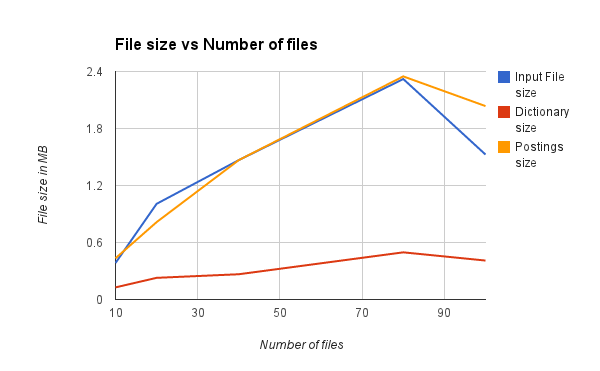
\includegraphics[width=.6\linewidth]{size_1.png}}
\subfigure[100, 200, 300, 400, 500]{ \label{fig:sub2}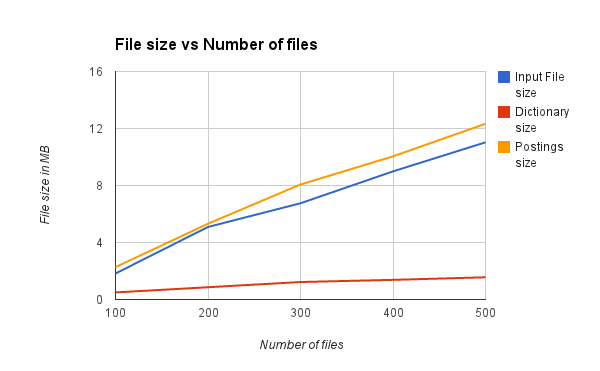
\includegraphics[width=.6\linewidth]{size_2.png}}
\caption{Size of files against number of documents}
\end{figure}

\clearpage

\begin{thebibliography}{1}

\bibitem{impj}Python nested dictionary http://stackoverflow.com/questions/635483/what-is-the-best-way-to-implement-nested-dictionaries-in-python

\bibitem{comp} http://nlp.stanford.edu/IR-book/html/htmledition/postings-file-compression-1.html

\bibitem{tuple} http://stackoverflow.com/questions/16302209/python-string-from-list-comprehension


  \end{thebibliography}

%%% End document
\end{document}